\documentclass{article}
\author{}

\usepackage{graphicx}
\usepackage{wrapfig}
\usepackage{enumerate}
\usepackage{hyperref}
\usepackage{float}
\usepackage[margin = 2.25cm]{geometry}
\usepackage[table]{xcolor}
\usepackage{fancyhdr}
\hypersetup{
  colorlinks = true,
  urlcolor = blue
}
\setlength\parindent{0pt}
\pagestyle{fancy}
\fancyhf{}
\rhead{College of Engineering, Construction and Living Sciences\\Bachelor of Information Technology}
\lfoot{Practical 09 Django 3: Forms \& Class-Based Views \\Version 1, 2020}
\rfoot{\thepage}

\begin{document}

\begin{figure}
	\centering
	
\includegraphics[width=50mm]{./img/logo.png}
\end{figure}

\title{College of Engineering, Construction and Living Sciences\\Bachelor of Information Technology\\IN608: Intermediate Application Development Concepts\\Level 6, Credits 15\\\textbf{Practical 09 Django 3: Forms \& Class-Based Views}} 
\date{}
\maketitle

\textbf{Due Date:} 31/08/2020 at 5pm \\

In this practical, you will complete a series of tasks covering today's lecture. This practical is worth 1\% of the final mark for the IN608: Intermediate Application Development Concepts course. \\

Before you start, in your practicals repository, create a new branch called \textbf{09-practical}.

\section*{Task 1} 
Create a Django project called \texttt{dog}. \texttt{cd} to \texttt{dog}, create a virtual environment \& install Django. Create an app called \texttt{practical09dogsearch}. Please ensure you configure your app in \texttt{dog/settings.py} \& \texttt{dog/urls.py}. In the \texttt{practical09dogsearch} directory, create a directory called \texttt{templates} \& sub-directory called \texttt{practical09dogsearch}. In \texttt{templates/practical09dogsearch}, create two \texttt{HTML} files called \texttt{index.html} \& \texttt{results.html}. \\

In \texttt{models.py}, copy \& paste the \texttt{Dog} model from the previous practical. \\

In \texttt{index.html}, create an \texttt{HTML} form. The form \texttt{action} should map to the \texttt{results} function in \texttt{views.py} \& the \texttt{method} should be \texttt{POST}. For adaptability, friendliness, grooming needs \& trainability, use radio buttons. For physical needs, use a select drop down. For each \texttt{HTML} form element, i.e., input \& select, set the \texttt{name} attribute to the appropriate \texttt{Dog} model field \& set the \texttt{value} attribute to the appropriate \texttt{RANGE\_CHOICE} actual value. Add a \texttt{submit input} below the mentioned elements. \\

In \texttt{views.py}, create a class called \texttt{IndexView} which extends \texttt{generic.TemplateView}. In this class, set the \texttt{template\_name} to \texttt{practical09dogsearch/index.html}. Create a function called \texttt{results}. In this function, you will query the \texttt{Dog} model using \texttt{filter} \& return a \texttt{QuerySet} containing objects that match the given lookup arguments. In this instance, the lookup arguments will be the items in \texttt{POST} request. Render the \texttt{details.html} template with a \texttt{context} dictionary containing the \texttt{QuerySet}. In \texttt{details.html}, if the \texttt{QuerySet} in \texttt{context} is not empty, display the length of the \texttt{QuerySet} \& \texttt{context} in a nicely formatted \texttt{HTML} table. If the \texttt{QuerySet} in \texttt{context} is empty, display an appropriate message. \\

Create a file called \texttt{urls.py} in the \texttt{practical09dogsearch} app directory. In \texttt{urls.py}, set the \texttt{app\_name} to \texttt{practical09dogsearch} \& create two URLs which map to the \texttt{IndexView} class \& \texttt{results} function in \texttt{views.py}.

\subsection*{Expected Output} 
Run the command \texttt{python manage.py runserver} then navigate to \href{http://127.0.0.1:8000/practical09dogsearch/}{http://127.0.0.1:8000/practical09dogsearch/} \\

\textbf{Note:} The user should be able to search on any combination of fields.

\begin{figure}[H]
  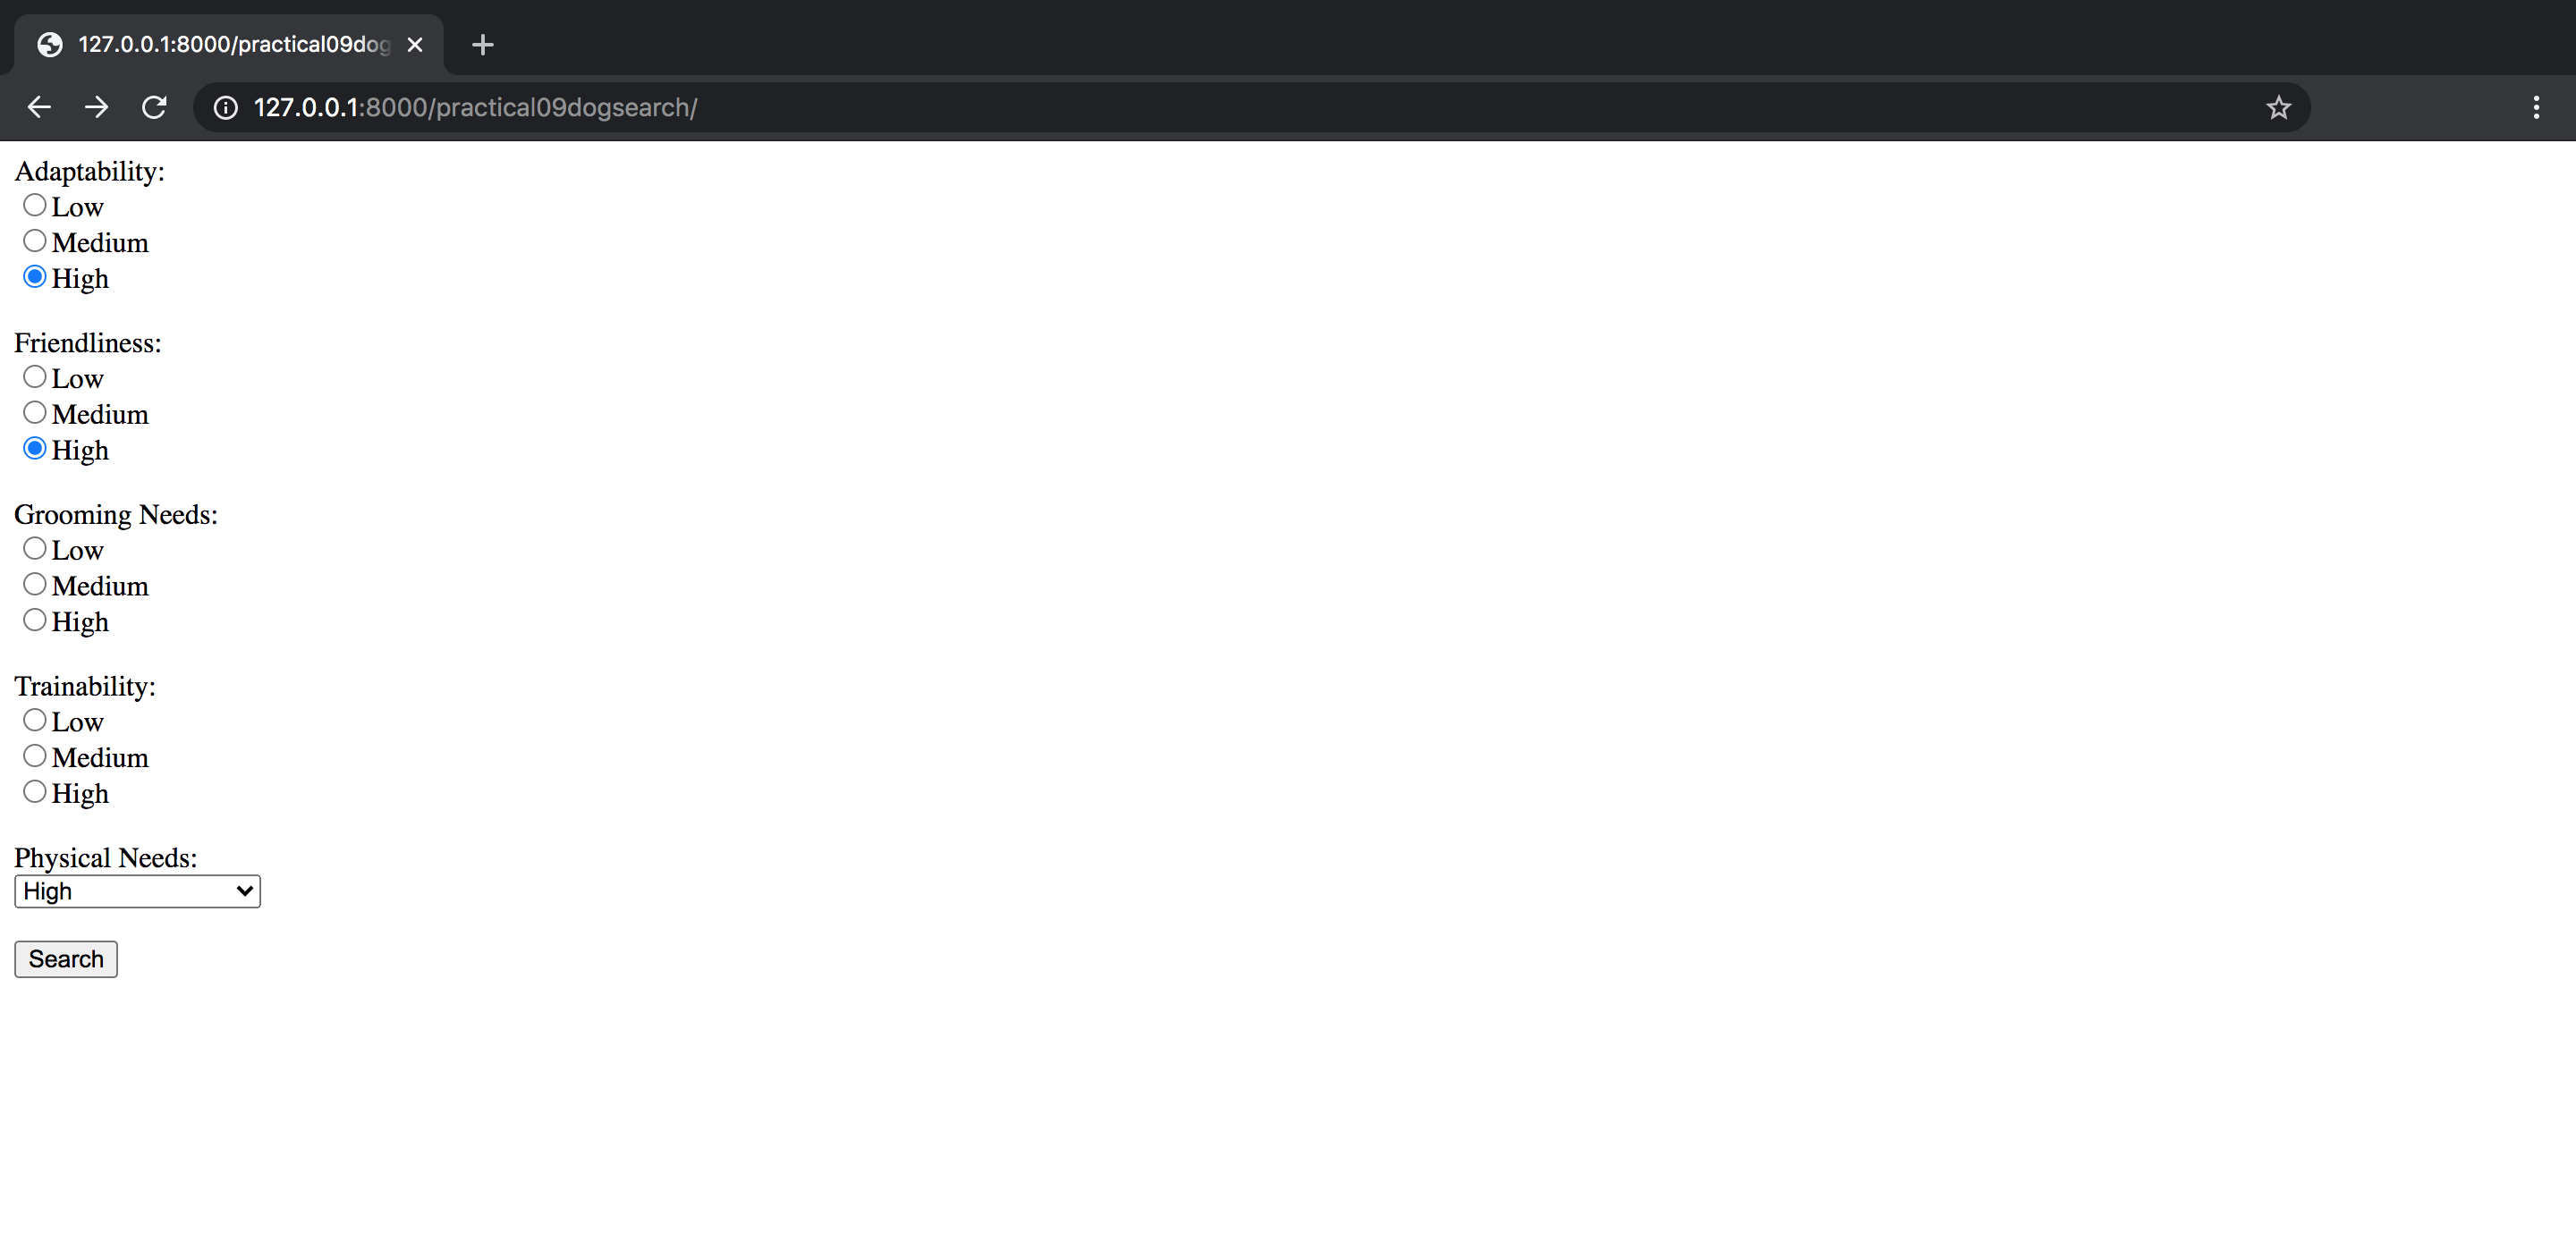
\includegraphics[width=175mm, height=85mm]{./img/09-expected-dog-selector-1.png}
\end{figure}

\begin{figure}[H]
  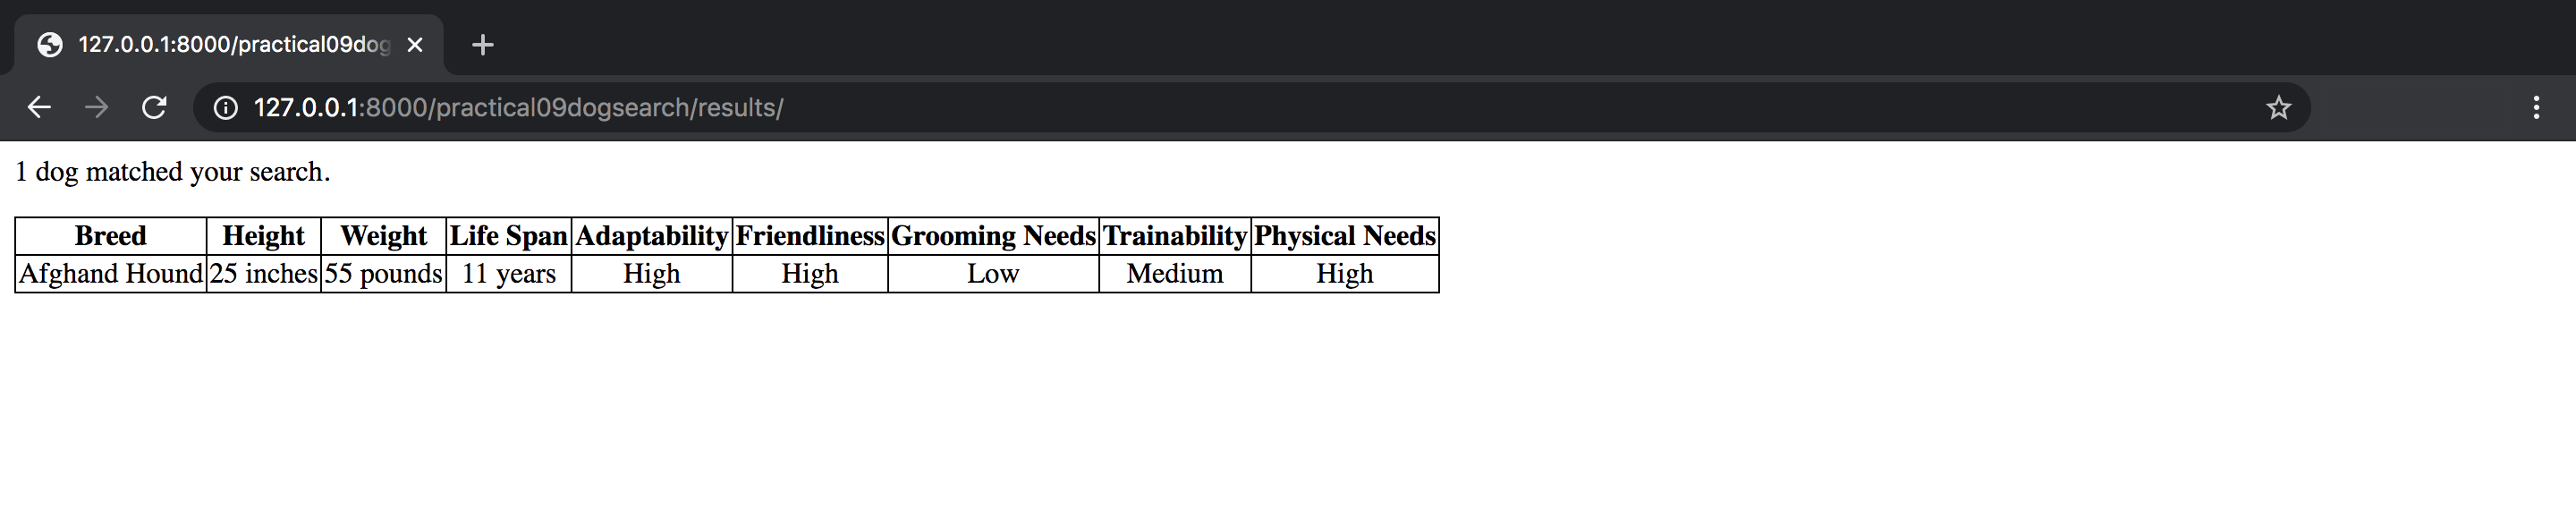
\includegraphics[width=175mm, height=35mm]{./img/09-expected-dog-selector-2.png}
  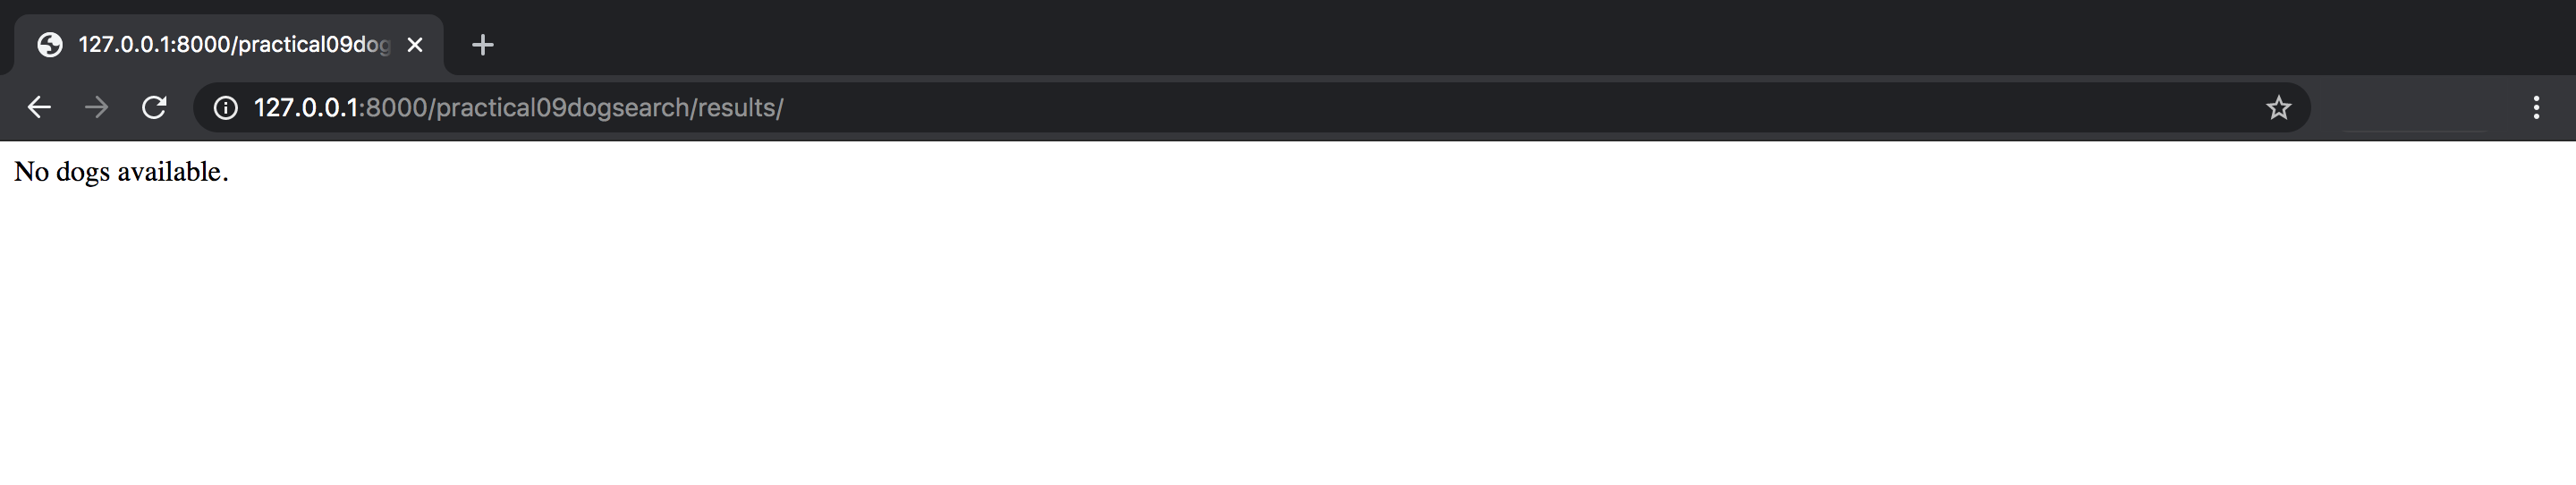
\includegraphics[width=175mm, height=35mm]{./img/09-expected-dog-selector-3.png}
\end{figure}

\textbf{Deployment link:} \href{https://int-app-dev-practical-09.herokuapp.com/practical09dogsearch/}{https://int-app-dev-practical-09.herokuapp.com/practical09dogsearch/}

\subsection*{Resources} 
\begin{itemize}
  \item \href{https://docs.djangoproject.com/en/3.0/topics/db/queries/}{Django Queries}
  \item \href{https://pypi.org/project/mysqlclient/}{MySQL Client}
\end{itemize}

\section*{Task 2} 
Create a Django project called \texttt{github}. \texttt{cd} to \texttt{github}, create a virtual environment \& install Django. Create an app called \texttt{practical09github}. Please ensure you configure your app in \texttt{github/settings.py} \& \texttt{github/urls.py}. In the \texttt{practical09github} directory, create a directory called \texttt{templates} \& sub-directory called \texttt{practical09github}. In \texttt{templates/practical09github}, create two \texttt{HTML} files called \texttt{index.html} \& \texttt{details.html}. \\

In \texttt{index.html}, create an \texttt{HTML} form. The form \texttt{action} should map to the \texttt{details} function in \texttt{views.py} \& the \texttt{method} should be \texttt{POST}. Add a \texttt{text input} with the \texttt{name} attribute value of \texttt{username} \& \texttt{submit input}. 
\begin{figure}[H]
  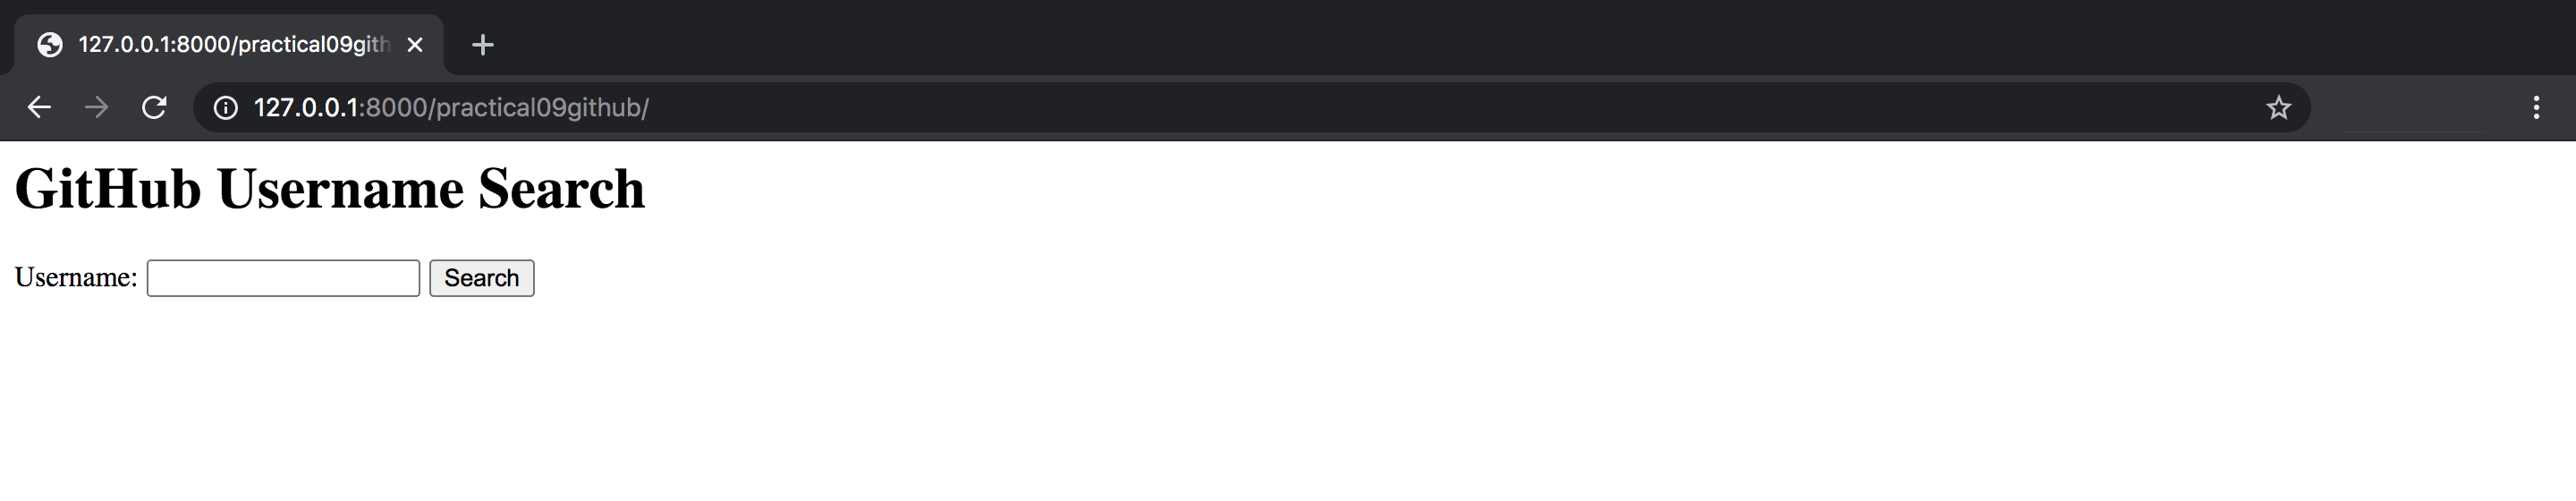
\includegraphics[width=175mm, height=35mm]{./img/09-expected-github-1.png}
\end{figure}

In \texttt{views.py}, create a class called \texttt{IndexView} which extends \texttt{generic.TemplateView}. In this class, set the \texttt{template\_name} to \texttt{practical09github/index.html}. \\

Create a function called \texttt{details}. In this function, get the \texttt{POST} \texttt{POST} \texttt{username} from the form. Use the \texttt{POST} \texttt{username} value \& make a \texttt{GET} request to \texttt{https://api.github.com/users/<username>}. \textbf{Note:} replace \texttt{<username>} with the \texttt{POST} \texttt{username} value. Please view the example response: \href{https://api.github.com/users/grayson-orr}{https://api.github.com/users/grayson-orr} \\

Create a dictionary called \texttt{context}. If a \texttt{POST} \texttt{username} value is found, add the response contents from the \texttt{GET} request to the dictionary. In addition, make another make a \texttt{GET} request to \texttt{repos\_url}. The response content will contain a list of repository information for that particular \textbf{GitHub} user. Add the response content to \texttt{context}. Please ensure correct error checking. \\

In \texttt{details.html}, display the \texttt{context} dictionary in the same format as shown in the expected output.\\

In \texttt{urls.py}, set the \texttt{app\_name} to \texttt{practical09github} \& create two URLs which map to the \texttt{IndexView} class \& \texttt{details} function in \texttt{views.py}.

\subsection*{Expected Output} 
Run the command \texttt{python manage.py runserver} then navigate to \href{http://127.0.0.1:8000/practical09github/}{http://127.0.0.1:8000/practical09github/} \\

\begin{figure}[H]
  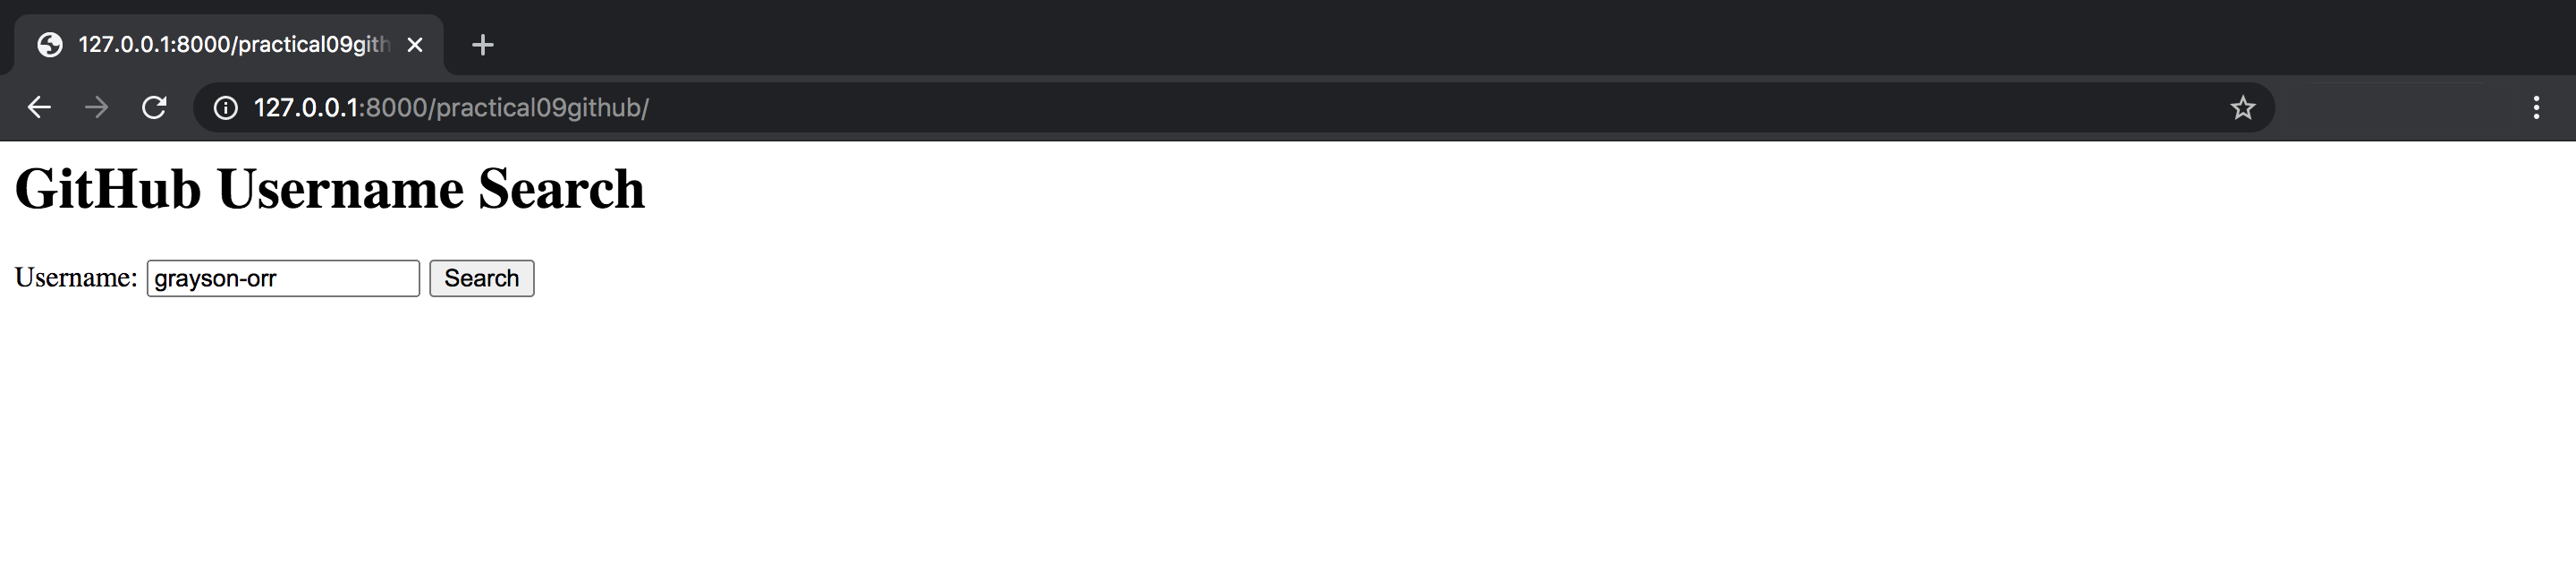
\includegraphics[width=175mm, height=35mm]{./img/09-expected-github-2.png}
  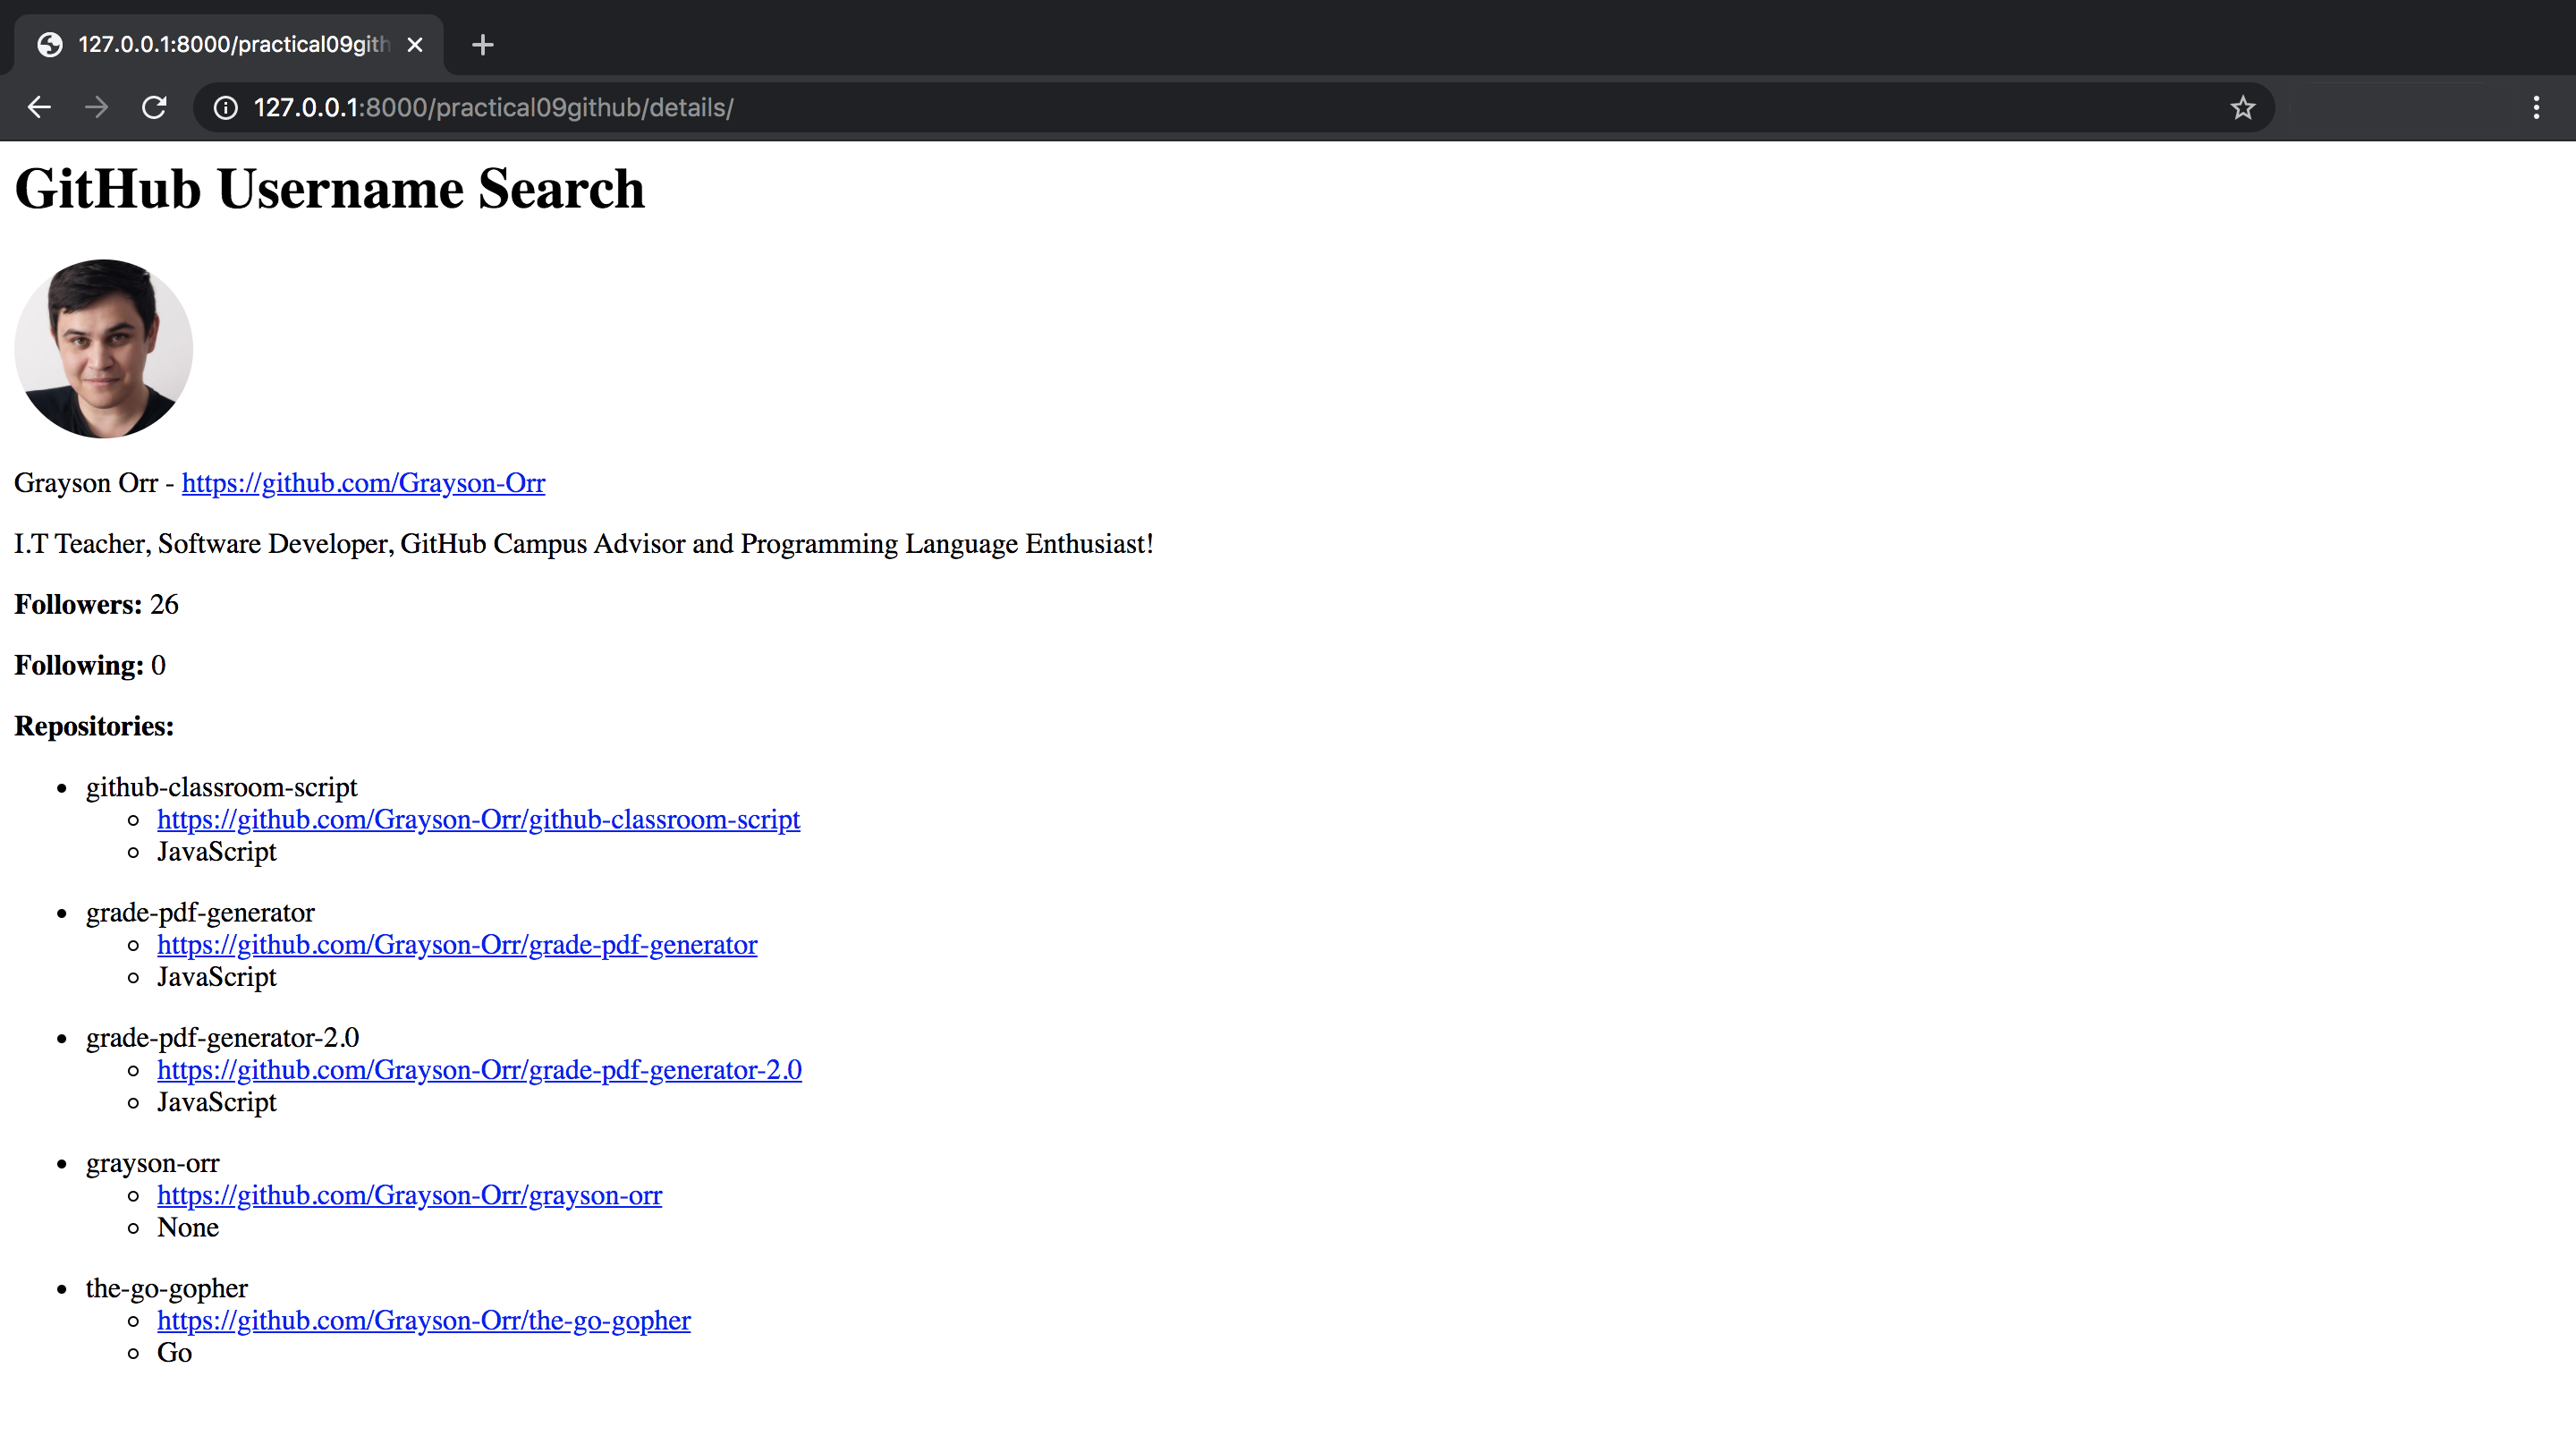
\includegraphics[width=175mm, height=100mm]{./img/09-expected-github-3.png}
\end{figure}

\begin{figure}[H]
  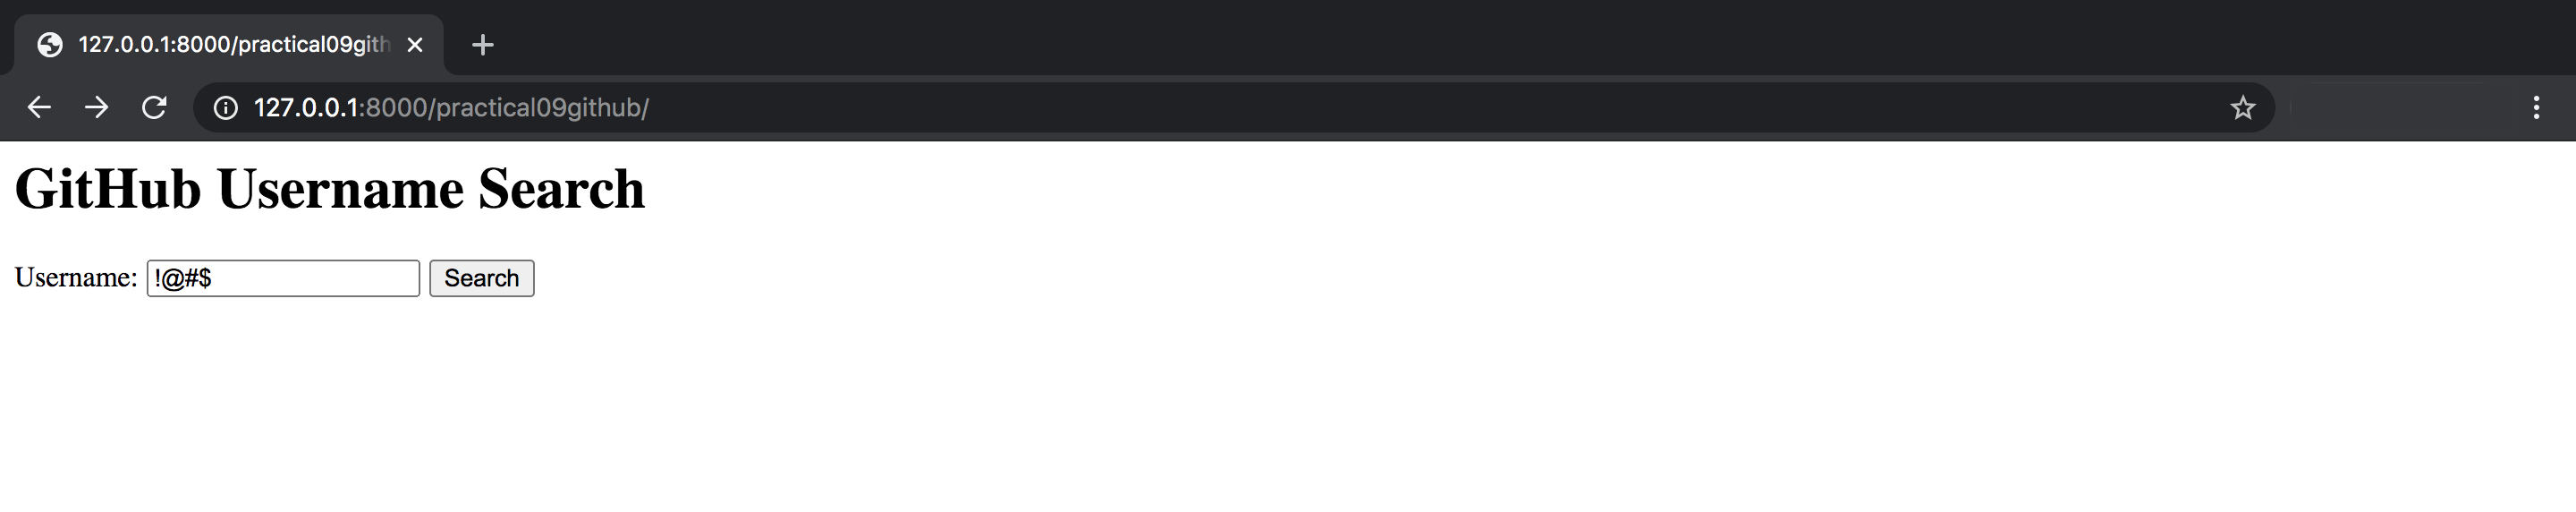
\includegraphics[width=175mm, height=35mm]{./img/09-expected-github-4.png}
  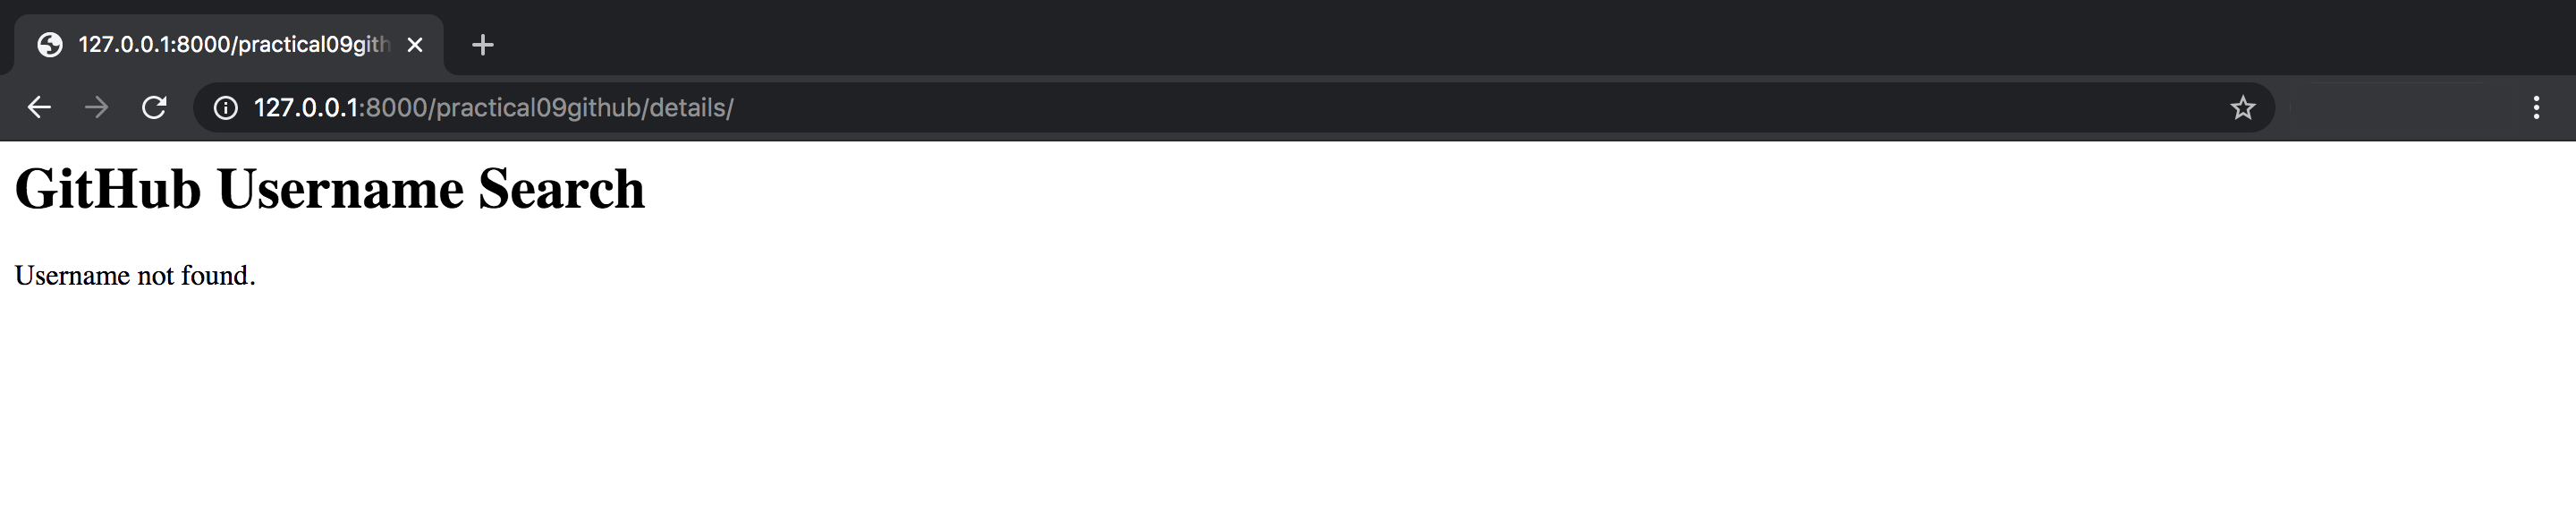
\includegraphics[width=175mm, height=35mm]{./img/09-expected-github-5.png}
\end{figure}

\textbf{Deployment link:} \href{https://int-app-dev-practical-09.herokuapp.com/practical09github/}{https://int-app-dev-practical-09.herokuapp.com/practical09github/}

\subsection*{Resources} 
\begin{itemize}
  \item \href{https://developer.github.com/v3/}{GitHub Developer API}
\end{itemize}

\end{document}